% A Theory section should extend, not repeat, the background to the
% article already dealt with in the Introduction and lay the
% foundation for further work.

\section{Background}
\label{sec: backg}
\subsection{PM Monitoring Sensors}

Despite their price, low-cost optical PM monitors have shown to be able to characterize PM concentrations with high resolution. Recent studies show that these perform with adequate precision for indoor air monitoring, although with some calibration requirements \cite{Manikonda2016}, having also demonstrated overall good correlations with reference monitors \cite{Sayahi2018}. Additionally, it has been concluded that comprehensive understanding of the sensor characteristics is necessary and that one big disadvantage is the non-guaranteed accuracy and the lack of established scientific literature regarding this equipment \cite{Kuula2019}.

Zheng et al., in 2018, tested how environment circumstances affect these sensors performance. Results showed that relative humidity (RH) has a major influence in the sensor readings, while the temperature effects were negligible \cite{Zheng2018}.

\subsection{Interpolation Algorithms for Spatial Analysis}

Spatial interpolation consists of estimating the value of measures of certain properties, at unsampled locations, within the area covered by existing observations of the same properties. Some of the most popular spatial interpolation models (SIM) are inverse distance weighting (IDW), kriging, shape functions, spline, and trend surface \cite{Li2008}.

In 2014, Li and Heap made a review of the 25 most commonly applied SIMs \cite{Li2014}. As result, an easy to use decision tree was created for use case dependent method selection. The most suitable interpolation algorithms in circumstances such as the ones in this work are IDW and ordinary kriging (OK), depending on data selection and availability, according to the decision tree.

\subsubsection{Fuzzy Boolean Nets}

FBNs are Boolean networks developed and studied by researchers at Instituto Superior Técnico \cite{Tome}. In these networks, each neuron has a binary value and is constituted by a binary table with a user-defined length. 

The networks are constituted by several neuronal areas. Each area has the same number of neurons and can only be one of two types, antecedent or consequent. 

Connections between neurons are weightless, temporary and only appear between neurons located in different areas of different types. In Figure \ref{fig:fbn-drawing}, a simple example of an FBN is presented, with two antecedent areas and one consequent area, each with four neurons.

\begin{figure}[ht]
\centering
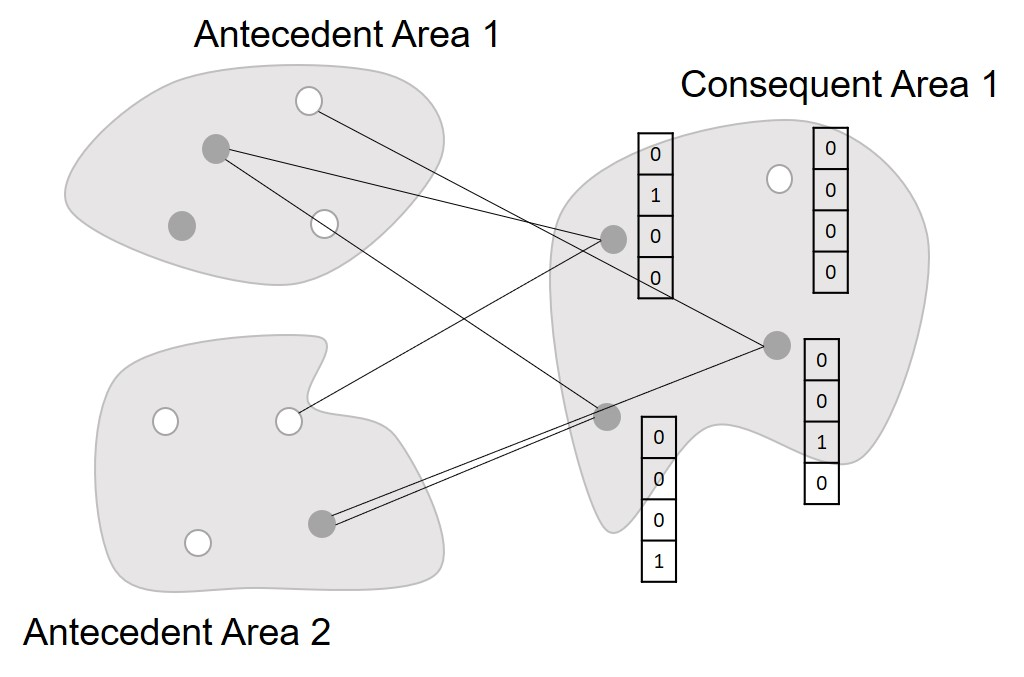
\includegraphics[width=0.45\textwidth]{./Images/fbn-drawing-2.jpg}
\caption{Example of the constituents of an FBN.}
\label{fig:fbn-drawing}
\end{figure}

The values of training and testing variables are attributed as an activation ratio to each area.

The inference process results of learning and testing epochs where consequent neurons sample an user-defined number of antecedent neurons, and according to these samples, fill their binary tables, in the training process, or retrieve a value from it, in the testing process. The final activation ratio of consequent areas represent the inference results. 

In previous studies, FBNs have shown to have positive interpolation capabilities when tested with sparse datasets \cite{Tome2014}.

\subsubsection{IDW}

IDW is a deterministic SIM based only on the assumption that the degree of influence of nearby sample points should be greater than the effect of farthest points. The only parameter which is user-defined in the IDW implementation is the power function, which defines the relevance of the distance in the calculation of the weights of each observed value \cite{Mesquita2009}.

The IDW interpolation can be defined by the equation \eqref{idw}, where \eqref{idw-weight} represents the weights associated to each observation.

\begin{equation} 
\label{idw}
\scalebox{1.2}{ $ f(x, y) = \dfrac{\sum_{i=1}^{n} w(d_i)z_i}{\sum_{i=1}^{n} w(d_i)}, i = 1, 2, ..., n$}
\end{equation}

\begin{equation} 
\label{idw-weight}
\scalebox{1.2}{ $w(d_i)= \dfrac{1}{{d_i}^{p}}$}
\end{equation}

Where $z_i$ is the observed value, $d_i$ is the distance between the estimation and the observation points, $w(d_i)$ represents the weight associated to observation \textit{i} and \textit{p} is the power function.

\subsubsection{Ordinary Kriging}

Kriging geostatistical schemes are stochastic, local, gradual and exact interpolators. In kriging, weights are based not only in the distance between points but also in the overall spatial arrangement of the observation points \cite{Mesquita2009}.

Before its application, an exploratory statistical analysis of data must be made, as well as the modelling of a variogram to represent how semivariance varies with distance.

In Figure \ref{fig:variogram}, an example of a variogram is presented. The nugget represents the semivariance value when the distance tends to zero. The sill is the point where semivariance stabilizes, and range is the interval in which, as distance increases, higher is the semivariance. Kriging interpolation weights are chosen using the modeled variogram so that estimates are unbiased and the estimation variance is minimized.

\begin{figure}[ht]
\centering
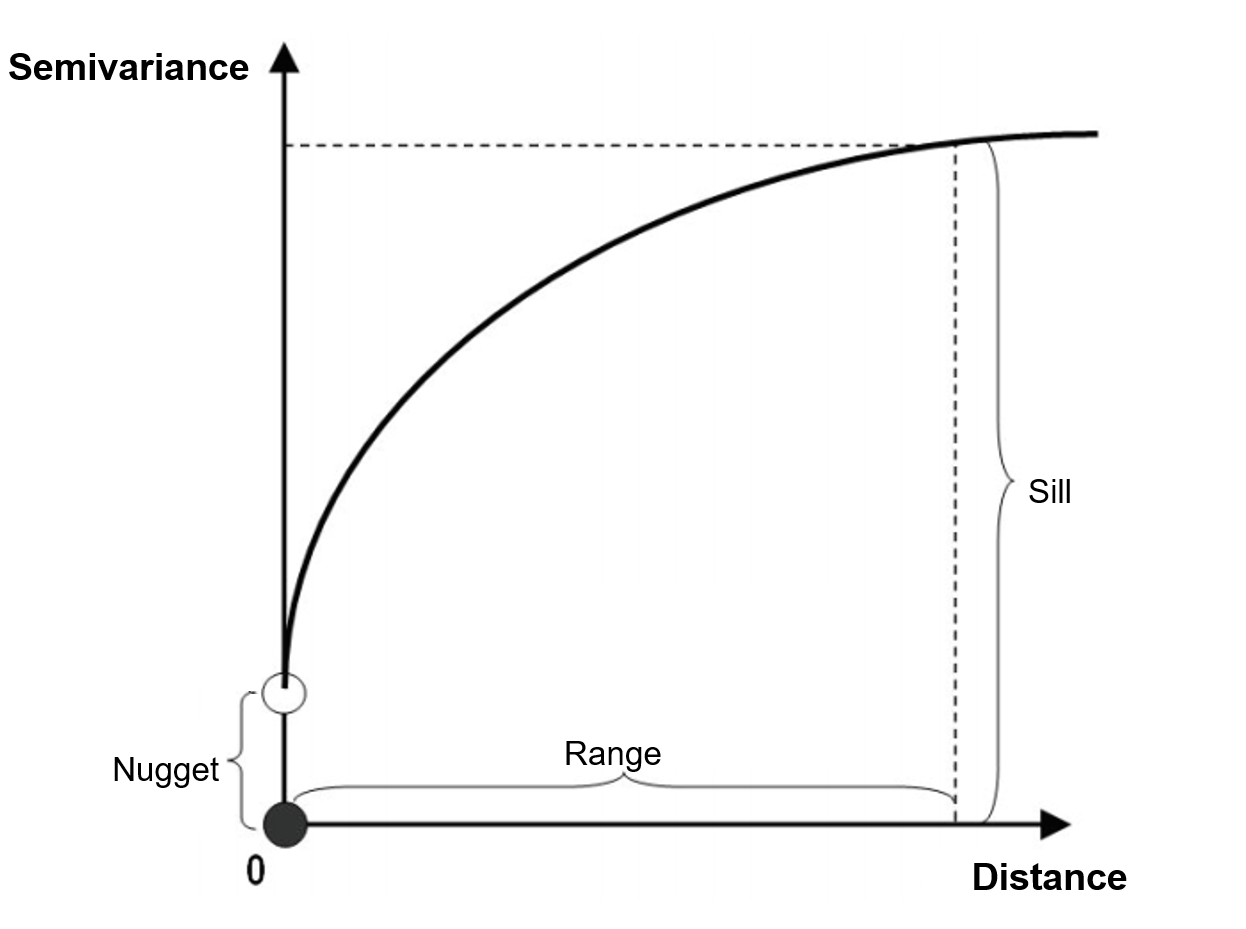
\includegraphics[width=0.49\textwidth]{./Images/variogram.png}
\caption{Example of a kriging variogram.}
\label{fig:variogram}
\end{figure}

\subsection{NB-IoT}

NB-IoT is a Low Power Wide Area Network (LPWAN) technology created in 2015 to face the growing massive IoT connectivity challenge. It operates on 180 kHz bandwidth for both downlink and uplink. The downlink remains with the same structure as Long Term Evolution (LTE) (orthogonal frequency-division multiple access (OFDMA) with 15 kHz sub-carrier spacing), and the uplink is single-carrier frequency-division multiple access (SC-FDMA) with sub-carrier spacing at 3.75 kHz (15 kHz for in-band to avoid interference from other LTE traffic) \cite{Ratasuk2016}.

Studies have compared NB-IoT to other LPWANs, such as SigFox, Long Term Evolution for Machines (LTE-M) and Long Range Wide Area Network (LORAWAN), and several advantages were observed over the latter. Some of these are that NB-IoT is more robust in terms of packet error rate \cite{Mroue2018}, it provides the best coverage, even in indoor scenarios \cite{Lauridsen2017}, and is the most suitable for IoT personal and public applications \cite{Zanella2016}.

\subsection{Air Pollution Visualization}

Currently there are two types of platforms for the visualization of live air quality data: governmental and private companies platforms.

Reviewed governmental platforms do not show fine interpolated data in their air quality live maps \cite{QualAr} \cite{U.S.EnvironmentProtectionAgency}. Instead, low resolution maps that do not show air quality variances between stations are presented. On the other hand, business oriented platforms take advantage of the publicly available air quality data provided by governments to make their live interpolated air pollution maps as a products. These represent maps with much finer resolution, but the algorithms used for the interpolation are proprietary \cite{Breezometer}.

